\documentclass[11pt,a4paper]{article}

\usepackage{lipsum}
\usepackage{graphicx}
\usepackage{subcaption}
\usepackage{fancyhdr}
\setlength{\headwidth}{16cm}
\pagestyle{fancy}
\usepackage[export]{adjustbox}

\usepackage{geometry}
\usepackage{amsfonts}
\geometry{
    a4paper,
    left=30mm,
    right=30mm,
    top=35mm,
    bottom=35mm,
    footskip=20mm,
    headsep=5mm,
    headheight=15mm}

%\usepackage{helvet}
%\renewcommand{\familydefault}{\sfdefault}
\renewcommand{\headrulewidth}{0pt}
\renewcommand{\footrulewidth}{0pt}
%\setlength\headheight{80.0pt}
%\addtolength{\textheight}{-80.0pt}
\fancyhead[R]{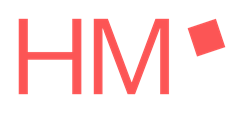
\includegraphics[width=4cm,right]{../HM-logo.png}}


\begin{document}

	\begin{center}
	%Hochschule für angewandte Wissenschaften München \\
	%Fakultät für Informatik und Mathematik
	Munich University of Applied Sciences \\
	\end{center}
	\vspace{1.5cm}
	%\\a
	\noindent\hrulefill
	\begin{center}
		\LARGE{\textsc{
			Uncertainty Estimation in Deep Reinforcement Learning\\
		}}
	\end{center}
	\vspace{0.1cm}
	\begin{center}
		\textsc{
			\Large{Research Report 1}
		}
	\end{center}
	\noindent\hrulefill
	\vspace{1cm}


	\begin{center}
		\small {on the research topic}\\
		\large{\textbf{
			Uncertainty Awareness and Risk Aversion\\in Deep Reinforcement Learning\\
		}}
	\vspace{2cm}
	\small{submitted by} \\
	\large{\textbf{Jonas Goltz}}
	\end{center}
	\vspace{7.5cm}


	\begin{center}
		\begin{tabular}{lll}
			\textbf{Study Course:} & &Master of Applied Research in Engineering Sciences\\
			\textbf{Department:} & &Computer Science and Mathematics\\
			\textbf{Submission Date:} & &10.02.2021\\
			\textbf{Supervisor:} & &Prof. Dr. David Spieler
		\end{tabular}
	\end{center}


%    \title{Uncertainty Awareness and Risk Aversion in Deep Reinforcement Learning}
%    \date{\today}
%    \author{
%        Jonas Goltz / Prof. Dr. Spieler \\
%        Fakultät 07\\
%        Hochschule München\\
%        goltz.jonas@googlemail.com\\
%        }
%    \maketitle
	\newpage

%    \begin{abstract}
%
%    \end{abstract}
	\tableofcontents
	\newpage

    \thispagestyle{fancy}


    \section{Introduction}\label{sec:introduction}
    \lipsum[1]

	\subsection{Motivation}\label{subsec:motivation}
	\lipsum[2]

	\section{Learning Frameworks}\label{sec:learning-frameworks}
	Reinforcement Learning (RL) is defined as learning through feedback from interacting with an environment.
	In this work we will only give a very brought overview of the general topic of RL as far as it is necessary to understand the adaption made for Deep Reinforcement Learning (DRL) and the implementation.
	We assume the reader to be familiar with the overall concepts of RL and Markov Decision Processes.
	For an introduction to RL we refer to Sutton and Barto~\cite{sutton_introduction_1998}.\\

	In general there are two different subtypes of RL algorithms, Policy Learning (PL) and Value Learning (VL).
	VL learns the expected value $v \in V$ as mapping $F: S \rightarrow V$ or $F: S \times A \rightarrow V$, with the state space	$S$ and the action space $A$.
	The policy $\pi$ is the derived from the estimated values using some heuristic as $\epsilon$-greedy or the softmax heuristic.\\
	In difference to that PL does not take the intermediate step of learning values, but directly learns the policy $\pi$ itself, approximating the mapping $F : S \times A \rightarrow [0, 1]$, represented as a probability distribution over the actions.
	This difference it crucial when it comes to exploration strategies, since it can be freely chosen in VL, but is inherent to the agent in PL.\\

	In general $F$ can be learned by any function approximator, in the most simple case of a small discrete state and action space this can even be done by a look-up table.
	In DRL a neural network is used as a function approximator, utilizing their extraordinary generalization and feature extraction capabilities even in high dimensional and continuous spaces.\\
	In the following sections we briefly introduce some of the most common learning frameworks used in DRL.

	\subsection{REINFORCE}\label{subsec:policy-gradient}
	The REINFORCE algorithm also know as Policy Gradient (PG) is part of the PL family.
	Generally spoken it uses the reward for an action to modify the probability distribution over the actions, actions that yield an higher reward become more likely while those less promising become less likely.
	The precise mathematics can be found in~\cite[Sutton]{sutton_introduction_1998} and~\cite[Williams]{williams_simple_1992}.
	Implementing the update function
	\[\theta \leftarrow \theta + \alpha \nabla \mathcal{L}\]
	with
	\[\nabla \mathcal{L} \approx \frac{1}{N} \sum^N_{i=1} \sum^T_{t=1} \nabla \log(\pi(a|s))\mathcal{R}\]
	with
	\[ \mathcal{R} = (\sum_{t'=t}^T r(s_{i, t'}|a_{i, t'})) \]
	where $\mathcal{R}$ is called the advantage.
	The REINFORCE algorithm can be stabilized by using a reward baseline, subtracting the expected reward from the actual received one, replacing the reward $\mathcal{R}$ with the so called advantage $\mathcal{R}'$
	\begin{equation}\label{eq:advantage}
		\mathcal{R}' = \sum_{t'=t}^T r(s_{i, t'}|a_{i, t'})) - \mathbb{E}[r(s, a)]
	\end{equation}
%	look this up the math looks somehow odd

	REINFORCE is an on-policy RL algorithm.

	\subsection{Deep Q-Learning}\label{subsec:deep-q-learning}
	Deep Q-Learning (DQN) was introduced by Mnih et al.~\cite{mnih_human-level_2015} and belongs to the family of VL algorithms, hence approximating the Q-Function $Q$ of a state-action pair.
	It does so by using Temporal Difference Learning (TD)
	\[Q(s,a) \leftarrow (1-\alpha)\, Q(s,a) + \alpha\,(r + \gamma \max_{a'}Q(s', a'))\]
	where $\alpha$ is the learning rate, $\gamma$ is the discount factor, $s'$ is the next state reached after taking action $a$.
	DQN belongs to the family of off-policy algorithms.
	
	\subsection{Double Deep Q-Learning}\label{subsec:double-deep-q-learning}
	Double Deep Q-Learning (DDQN)~\cite{van_hasselt_deep_2015} is a derivation of the DQN framework.
	In difference to standard DQN it uses its property as an off-policy algorithm implementing replay memory and in addition a so called target network.
	The replay memory is used to store previous experiences to learn from.
	Each iteration, the agent updates a part of the memory with new episodes and then samples from its memory to update it weights.
	This decouples the memories used in a forwad pass, which stabilizes the learning process and increases the sample efficiency, since the agent can learn from the same memory multiple times.
	Replay memories have the drawback that they can only be used by an off-policy algorithm as DQN.\\

	In addition DDQN uses a target network parametrized by $\theta'$, which is used to evaluate the Q-Function for the next state $s'$.
	Hence, the update function becomes
	\[Q(s,a) \leftarrow (1-\alpha)\, Q(s,a) + \alpha\,(r + \gamma \max_{a'}Q'(s', a'))\]
	where $Q'$ is parametrized by $\theta'$.
	In the default implementation $\theta'$ is periodically set to $\theta$ every couple of iterations, but it can also be dragged behind the main network with the update rule.
	\[\theta' \leftarrow (1 - \delta) \theta' + \delta \theta\]
	where $\delta \in [0,1]$ is the update fraction for the target network.
	This stabilizes learning by fixing the target Q-values for several consecutive steps, therefore making it easier for the network to learn.

	\subsection{SARSA}\label{subsec:sarsa}
	SARSA, as introduced by Sutton~\cite{sutton_introduction_1998}, also belongs to the family of VL, but in difference to DQN it is a on-policy algorithm, implementing the update function
	\[Q(s,a) \leftarrow (1-\alpha)\, Q(s,a) + \alpha\,(r + \gamma Q'(s', a'))\]
	where $a'$ is the actual taken action in the new state $s'$, which gives the name State Action Reward new State new Action.
	Interestingly, regardless of its on-policy property, it can be implemented using a replay memory, as long as  old memories are replaced recently enough so that the weights have not diverged too much from those, when the memory was collected.\\
	The SARSA framework has the interesting property of being able to incorporate aleatoric uncertainty into the learning process, therefore avoiding potentially risky situations as shown by Sutton~\cite{sutton_introduction_1998}.

	\subsection{A3C}\label{subsec:a3c}
	The Asynchronous Advantage Actor Critic (A3C) by Mnih et al.~\cite{mnih_asynchronous_2016} is an extension of the actor-critics algorithm by Konda et al.~\cite{konda_actor-critic_2000}.
	The fundamental idea of actor-critics algorithms is to replace the advantage~\ref{eq:advantage} by a learned function approximation, in other words a DQN in the setting of DRL.

	\section{Uncertainty}\label{sec:uncertainty}
	There are two different types of uncertainty in Reinforcement Learning.
	Aleatoric uncertainty arising from the uncertainty/stochasticity of the environment.
	Epistemic uncertainty arises from the uncertainty of the learning process.
	Differentiating between the two of them is important, since e.g. even an infinitely powerful learner, will only be able to prevent epistemic uncertainty, but can never reduce aleatoric uncertainty.
%	Write some more about it and why this is important, also cite some source

	\subsection{Uncertainty Estimation}\label{subsec:uncertainty-estimation}
	In modern RL and DL there are several ways of approximating and adjusting for uncertainty, but not all of those methods developed for either of them are applicable for DRL.
	The most commonly used approaches of uncertainty estimation in DLR, essentially boil down to different versions of ensemble methods.
	The following sections introduce three different types of uncertainty estimation in DL, which are applicable to RL.

	\subsection{Ensemble}\label{subsec:ensemble}
	Ensemble methods are a commonly used approach in which several usually weak learners are combined to obtain a strong learner.
	When using it in the context of DL an ensemble usually refers to a set of models, that were trained on different folds of the same data, aggregating their predictions either by averaging over the models or by applying a majority vote.
	When aggregating the models you can either estimate a variance over the prediction when using the average, or computing the entropy in case of a majority vote.
	For the sake of simplicity we refer to both, variance and entropy, as variance.
	In the context of DRL, ensembling means to train multiple agents on the same environment using different replay memories for each individual agent.

	\subsection{MC-Dropout}\label{subsec:mc-dropout}
	MC-Dropout as introduced by Gal et al.~\cite{gal_dropout_2016}, takes the point of view of dropout as an infinite ensemble technique where the different models of the ensemble share certain sections of their weights.
	In MC-Dropout one uses the dropout not only during training but also during inference, propagating the same input through different sub-graphs of the model.
	The obtained multiple predictions on the same output can then be aggregated in the same way as for a regular ensemble.

	\subsection{Bootstrapping}\label{subsec:bootstrapping}
	In standard Machine Learning, bootstrapping refers to resampling your data with replacement, to train multiple models each on its individual resampled data set.
	In DL bootstrapping is implemented in a slightly different way as introduced by Osband et al.
	~\cite{osband_deep_2016}.
	Instead of using several independent models, bootstrapping in DL means to train several models with a common core, but multiple heads each on different subsets of the data.
	This minimizes the computation computational costs, by a single forward pass through the core, with only the multiple heads increasing the computational complexity.

	\section{Implementation}\label{sec:implementation}
	In this section we will focus on the technical implementation of the learning frameworks and certainty evaluation methods mentioned before.

	\subsection{Tensorflow vs. PyTorch}\label{subsec:tensorflow-vs.-pytorch}
	There are two main frameworks to work with in DL, Tensorflow developed by Google and PyTorch developed by facebook.
	For this section we will focus on the aspects which are important when developing Neural Networks and neglect aspects relevant for deployment.\\

%	static vs dynamic
	Both of them are highly performant and much used frameworks but they take a different approach in the backend.
	While Tensorflow compiles to a single C or CUDA block, PyTorch uses the approach of a script language only calling C and CUDA routines.
	From that follows, that Tensorflow works with static, pre-compiled graphs, while PyTorch is able to work with entirely dynamic graphs, that can be change anytime during runtime.
	Though the dynamic of PyTorch comes with the disadvantage of a slightly worse performance in term of run time, making PyTorch slower then Tensorflow.\\

%	device
	Another difference is the device handling where PyTorch gives you full control over the device to be used for code execution, meaning that you can switch back and forth between the CPU and potentially multiple different GPU in a single forward pass, while Tensorflow defines the device for the entire session.
	This might not seem to be a fundamental difference, but it can have advantages over being fixed on a single device.
	Though, it comes with the drawback of the necessity to handle the devices manually, which we will come back to later.\\

%	debugging
	Having a dynamic graph as PyTorch has a large advantage when it comes to debugging.
	Essentially you have access to all tensors all the time during the execution, it is even possible to step through every single step of the forward pass by setting breaking points.
	Unfortunately, this is not possible with Tensorflow, which essentially is a black box with very limited access, making debugging a very tedious process.
%	Visulization
	Tensorflow counters that problem by providing a very handy visualization tool called tensorboard, which enables you to plot distributions and metrics during runtime.
	PyTorch itself does not provide a tool like that by itself, but there are similar tools that can be used with PyTorch.\\

%	Tedious code
	One disadvantage of Tensorflow is the sometimes tedious handling of input tensors and sessions.
	For this reason Tensorflow introduced the keras framework, a wrapper around tensorflow taking over most of the tensor and session handling necessary in Tensorflow.
	Though, it comes with disadvantages when it comes to more complex network architectures, while not solving the black box problem mentioned before.
	Unfortunately, PyTorch has no similar wrapper abstracting the learning frameworks, an aspect which we will come back to in section~\ref{subsec:pymatch}.\\

	Since we are not working with extremely large models for which runtime might become an important factor, we value flexibility and access to the model over speed, hence choosing PyTorch as our framework.\\

	\subsection{PyMatch}\label{subsec:pymatch}
	In this project we work with multiple different DRL frameworks and a couple of different uncertainty estimators in combination with a number of different environments.
	This makes it a very tedious and error-prone work to implement all learning frameworks with the different uncertainty estimators, where the same code snippets have to be written over and over again.
	As mentioned before PyTorch has no abstraction layer for learning frameworks as rudimentary provided by keras for Tensorflow, for which reason we introduce PyMatch, a learning framework abstraction build around PyMatch.
	In difference to keras PyMatch does not solely aim to take over the tedious data- and graph-handling as keras does, but it is meant to abstract the learning framework in a modular way, while not restricting the model architecture in any way.
	The core idea of PyMatch is to build everything from exchangeable modules using a fixed interface between them, making code as reusable as possible.\\

	\subsubsection{Learner}
	The fundamental abstraction core of PyMatch the the so called Learner.
	A Learner is simply a hull around a network (torch.nn.Module), a dataloader, a loss function and an optimizer.
	As with keras a Learner provides a fit() method, that trains the model on the provided data with the the given loss and optimizer.
	It also provides an easy way of storing and loading your model, including the optimizer and the loss, restoring their states.
	It also holds a member train\_dict which can be used to store all kinds of metrics and values over the training process.
	This train\_dict is also stored and loaded automatically, which frees the user of annoying and unnecessary data-loss or juggling saving and loading operations all over the learning script.
	In addition Learners can be moved and trained on devices, so the tiresome swapping of variables from and to devices is handled by the Learner itself.
	Each learning task can be implemented as a Learner, for this project it means that all learning frameworks mentioned in~\ref{sec:learning-frameworks} as its own Learner implementation, building upon each other.

	\subsubsection{Reinforcement Learners}
	Since this work is focussing on DRL we will describe the DRL Learners, also called Agents, in more depth.
	For the most simple DRL Agents, there are just few changes to make.
	First, instead of a standard data loader as in data driven learning frameworks, Agents have a memory, an environment they are interacting with and an action selection strategy.
	Memories provide the same interface as standard data loaders, but they are meant to change over time.
	In addition they provide additional functionality as storing and discounting rewards.
	They also have a defined length and refresh rate.
	The second change made for Agents is that they define they way how the agent interacts with their environment.
	This includes the way they interact, select their actions based on their strategy and the way they store memories.
	We have implemented all learning frameworks mentioned in~\ref{sec:learning-frameworks}, building upon the general Learner as well as on eachother\\
	
	
%	environments
	For our Agents we have chose to follow the interface implemented by the popular openAI gym~\cite{openai_gym_nodate} environments.
	This means that our agents work with any environment that implements the same interface without any further adjustments.
%	action selection
	For action selection we have implemented several different strategies.
	\begin{itemize}
		\item A greedy action selection, which is primarily used for evaluation purpose
		\item An $\epsilon$-greedy approach, taking a random action with the probability $\epsilon$
		\item A what we call distributional action selection, assuming a discrete or continuous probability distribution over the actions to sample from, as used for a Policy Gradient
		\item A softmax action selection, controlled by a temperature parameter, which can be used with all kinds of value based agents
		\item Thompson sampling, assuming a set of values with a confidence bound, sampling them for the respective Gaussian distribution
	\end{itemize}
	Those strategies can be used in any combination with our agents, though not all possible combinations make sense mathematically.
	For example combining a Policy gradient with a $\epsilon$-greedy-action selection is not a reasonable thing to do.

	\subsubsection{Experiments}
	PyMatch provides a very simple experiment documentation class, which exist in two versions: a homebrew one, storing everything on your local machine and one that uses the weights and bias (wandb) interface, monitoring even the hardware of your machine.
	Though to use wandb you need to create your own account.
	PyMatch Experiments are designed to be used with three files defining the experiment:
	\begin{enumerate}
		\item a model-file: This file contains the nn.Module only requiring a defined foward() method
    	\item a factory-file: This file contains a factory method for the Learner, i.e. it defines how the Learner is created which loss and crit are used etc.
    	\item a parameter-file: This file defines all additional hyper-parameter that are necessary to create and train the model
	\end{enumerate}

	All three files can be easily loaded by a simple call of the Experiment class, provided by PyMatch.
	Using this structure enables the user to use a single training script for all experiment runs and it ensures that an experiment always stays reproducible.
	In addition the Experiment class can store the training script in the experiment folder, by a single method call.

	This structure is particularly useful when running multiple experiments with different architectures and hyper-parameters and is required when using the Ensemble class provided by PyMatch

	\subsubsection{Ensembles}
	Abstracting learning frameworks and concepts with a standardized interface, as done by the Learner approach we take, has a big advantage when it comes to ensemble methods.
	In principle the Ensemble is just a wrapper around a list of Learners, but it also has its own loading and storing method, its own train\_dict and callbacks.
	When using the experiment structure as suggested above there is nearly no adjustment to make to go from a single Learner to an ensemble of Learners.
	Though, using an ensemble disables you to work with wandb, since wandb is only able to store weights and metrics for a single model, but not multiple models wrapped in a single one (though you could store all of them individually).

	The Ensemble comes with a KFold data folder, that can be used in the factory.
	The Ensemble can also be used to easily implement Neural Network Boosting and automated hyper-parameter searches, if the factory of the ensemble is randomized or used with a predefined set of different hyper-parameters.

	Ensembles provide the same fit() method as Learners do, but they can either train the Learners one by one or partition the training of the Learners.
	After each of those partitions the callbacks of the ensemble are called, e.g. this can be the evaluation of the ensemble as a whole, or to plot metrics from the learners or the ensemble.

	\subsubsection{Hats}
	Hats are meant to be placed on the head of a network or ensemble.
	The idea is to keep the aggregation and handling of the models output as flexible as possible.
	Hats can also be stacked on the head of a network only requiring that the output and input of consecutive hats match.
	This is particularly useful when dealing with ensembles, for either the aggregation of the different models or certainty estimations on the predicted values (e.g. estimating the standard deviation or the entropy).
	Hats are usually not part of the training process but could be incorporated in the Learner as well.
	
	\subsubsection{MC-Dropout}
	Implementing Dropout using PyMatch is a straight forward thing.
	There are only three minor adjustments you have to make compared to a standard Learner.
	First you have to redefine the eval-function of the PyTorch Module, to activate Dropout during evaluation.
	Second you have to stack the input $n$-times, where $n$ is the number of evaluations to be run.
	Last you have to use a reduction hat of choice - for example averaging or voting - to reduce the output of the model back to the original shape.
	
	\subsubsection{Boosting}
	We implemented Boosting as an ensemble of Agents sharing the common network core, using this approach we can nearly entirely rely on our Ensemble implementation with minor adjustments of our model factory.
	This includes a learning rate reduction on the common core by the factor $\frac{1}{n}$, where $n$ is the number of heads of the boosting algorithm.

	\section{Evaluation}\label{sec:evaluation}
	This work puts most focus on uncertainty estimation and the approaches it is based on.
	Therefore, we do not excessively compare the different learning frameworks, as they are generally highly dependent on the environments they are used with.
	The three main approaches to uncertainty estimation in Deep Reinforcement Learning are MC-Dropout introduced by Loquercio et.al ~\cite{loquercio_general_2020}, Bootstrapping as suggested by Osband et al.~\cite{osband_deep_2016}, as the third approach we use the commonly used model averaging, also known as ensemble method.\\
	For our evaluation we focus on two simply environments provided by OpenAI gym~\cite{openai_gym_nodate}, namely CartPole and the discrete version of LunarLander.\\

	Comparing RL algorithms with each other is not as straight forward as it usually is with standard ML.
	The reason for this is that RL typically has a much higher variance compared with data driven approaches and runs the risk of catastrophic forgetting.
	In addition many environments are stochastic, meaning that the same policy might lead to very different performance.
	To take the high variance into account we use a similar approach as Sutton and Barto~\cite{sutton_introduction_1998} evaluating models based on $k$ runs of the same agent, averaging the performance of all agents over each epoch.
	Since we are interested in the performance compared to the `average` model, we slightly modify the approach taken by Sutton and Barto by use the median instead of the mean.
	All performances are reported on the learned optimal policy, meaning that a greedy action selection strategy is used during evaluation.

	\subsection{Comparing uncertainty estimators with agents} \label{subsec:comparing-uncertainty-estimators-with-agents}

	\subsection{Ensemble}\label{subsec:ensemble2}
	When comparing ensembles with their baseline
	\begin{figure}
		\label{fig:ddqn_cartpole_ensemble}
		\centering
		\includegraphics[width=0.8\linewidth]{../../dqn/cartpole/ensemble/exp_39/avg_ensemble_val_rewards.png}
		\caption{DQN ensemble on a CartPole environment using multiple memories}
	\end{figure}

	\begin{figure}
		\label{fig:ddqn_cartpole_ensemble_single}
		\centering
		\includegraphics[width=0.8\linewidth]{../../dqn/cartpole/single_memory_ensemble/exp_55/avg_ensemble_val_rewards.png}
		\caption{DQN ensemble on a CartPole environment using a single memory}
	\end{figure}

	\subsection{Boosting} \label{subsec:boosting}
	\begin{figure}
		\label{fig:dqn_cartpole_boosting}
		\centering
		\includegraphics[width=0.8\linewidth]{../../DQN/CartPole/boosting/exp_58/avg_ensemble_val_rewards.png}
		\caption{DDQN ensemble on a CartPole environment}
	\end{figure}

	%! Author = Jonas
%! Date = 12.11.2020

\section*{Abbreviations}
\begin{tabular}{l l}
    \label{tab:table}
    DRL     & Deep Reinforcement Learning\\
    DQN     & Deep Q-Learning\\
    DDQN    & Double Deep Q-Learning\\
    ML      & Machine Learning\\
    PG      & Policy Gradient\\
    PL      & Policy Learning\\
    RL      & Reinforcement Learning\\
    TD      & Temporal Difference Learning\\
    VL      & Value Leargning\\
\end{tabular}

	%! Author = Jonas
%! Date = 12.11.2020

\section{Symbols}\label{sec:symbols}
\subsection{Reinforcement Learning}\label{subsec:reinforcement-learning}
\begin{tabular}{l l}
    $A$     & Action space\\
    $a$     & Action\\
    $\alpha$    & Learning rate\\
    $\gamma$    & Discount factor\\
    $\pi$   & Policy\\
    $Q$     & Q-Value function\\
    $r$     & Reward\\
    $S$     & State space\\
    $s$     & State\\
    $\theta$    & Parametrization of a function approximator\\
    $V$     & Value space\\
    $v$     & Value of a state\\
\end{tabular}

	\bibliography{references}
	\bibliographystyle{plain}
\end{document}

